\documentclass[../Results.tex]{subfiles}
\begin{document}
	Fig. \ref{overlayspec} shows the HST image of MAMMOTH-1 with WFC F160W filter with contours for Ly$\alpha$ HeII and CIV emission. All sources marked here are at z=2.3 confirmed by CO(1-0) emission(\cite{emonts2019cold}) and CO(3-2) emission(Qiong (in prep)). It shows Ly$\alpha$ emission extended $>20"$ which corresponds to $\approx170$kpc, this is the typical size of halo at this redshift. It covers all 8 sources here, this indicates that all of this sources could have contribution to illuminate this nebulae. Size of this nebulae is limited by the FoV of KCWI which is $20" \times 16.8"$ and is not sensitive enough at the edges. Furthermore, we clearly see that there are three peaks around Source-B, two out of the three peaks are on both sides of the G-5 respectively(Fig.\ref{kinematicsmap}). Besides, HeII and CIV emission also show extent signals(>$3\sigma$) which extend to $\approx 10"$ (physical projected scale of 85kpc) in the north-south direction(CIV emission even cover G-5).
	
	Fig. \ref{overlayspec} shows spectra extract in 1 $arcsec^{2}$ aperture centering on the flux peaks. We fit the three emission lines with single component gaussian function and also use the central wavelength fitted to calculate their redshifts, moreover we calculate their luminosity beyond $3\sigma$. We show these results and the fitting parameters in Tab. \ref{fit_L}. 
	\begin{figure*}
		\centering
		\subfloat[contour]{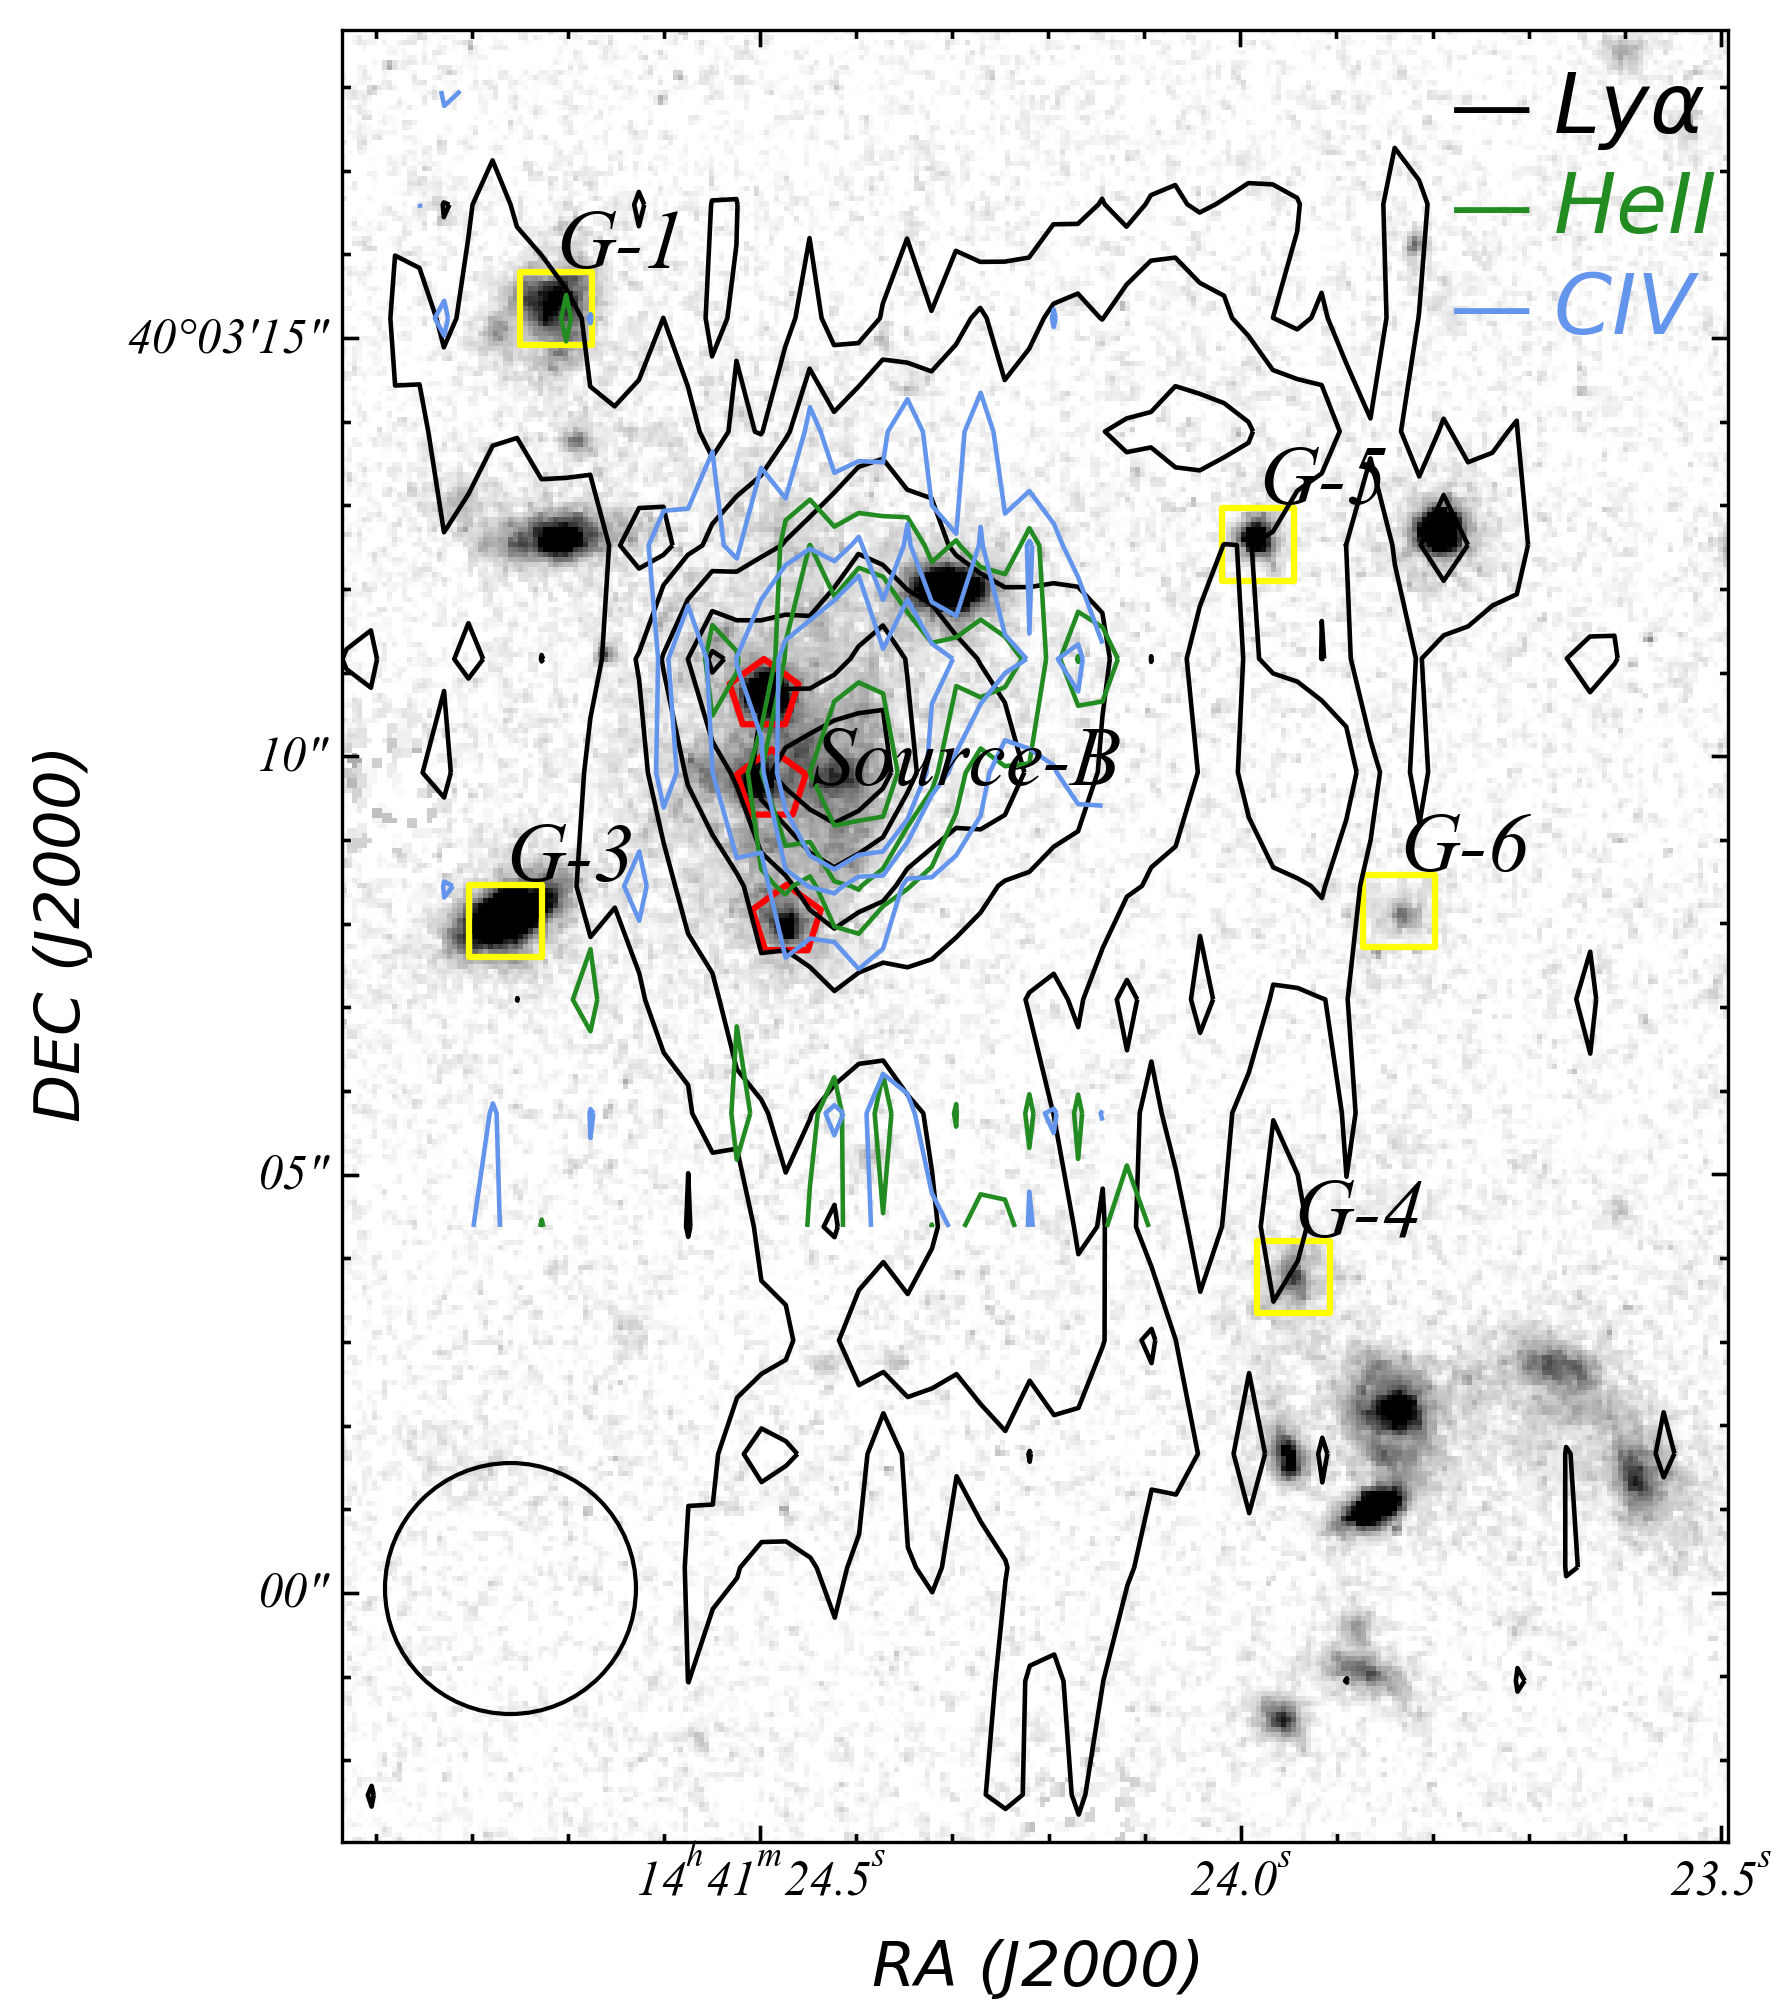
\includegraphics[width=0.5\textwidth]{figs/contour}}
		\subfloat[spectra]{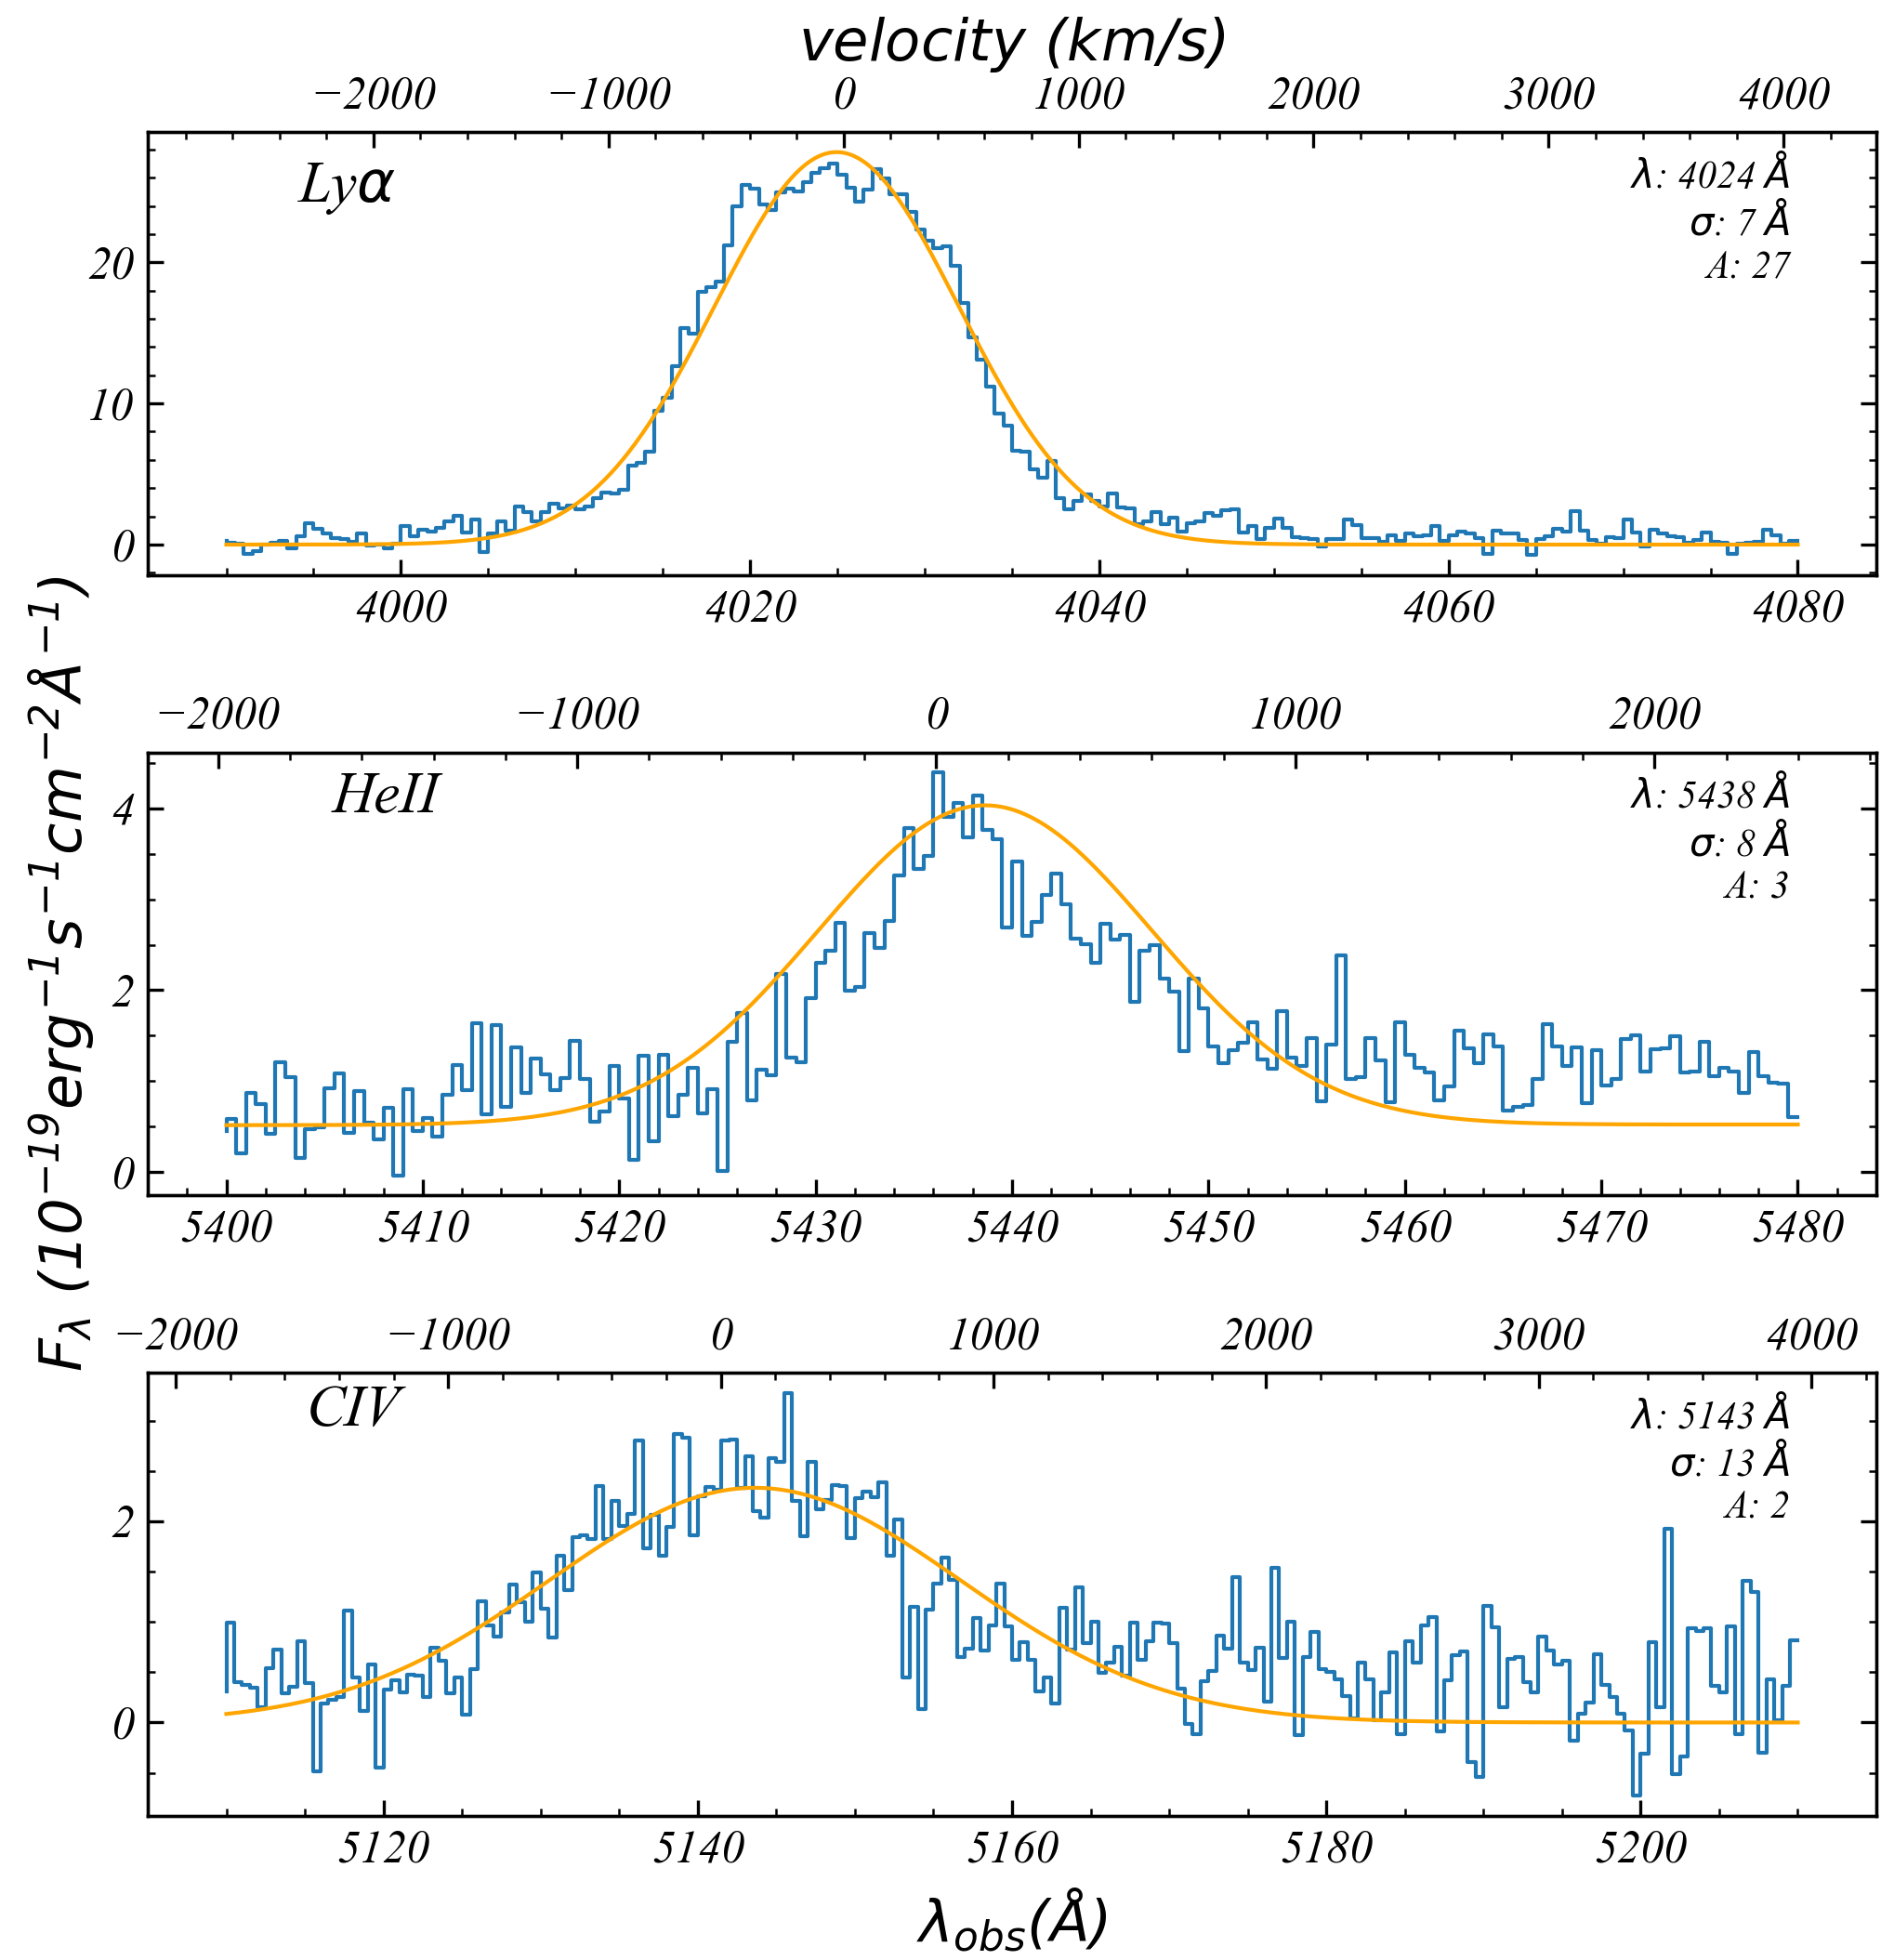
\includegraphics[width=0.5\textwidth]{figs/spectral}}
		\label{overlayspec}
		\caption{Left: HST image of MAMMOTH-1 from circle 24,25, PI: Cai. We overlay on it Ly$\alpha$ HeII and CIV psudo narrow band images. Black contour is Ly$\alpha$, blue contour is HeII, green contour is CIV. We also mark source-B with red mark and sources at the same redshift with yellow mark. We also plot circle with raidus of 1$arcsec^{2}$. Right: spectra of the 3 emission lines extracted from aperture center on source-B with radius 1$arcsec^{2}$, we fit them with one-component gaussian function.}
	\end{figure*}
	\begin{table}[htp]
	\begin{center}
		\begin{tabular}{ccccc}
\hline
\hline
& $\lambda_{c}(A)$ & $\sigma_{\lambda}(A)$ & L(erg/s) & redshift \\ \hline
Ly$\alpha$ &   4024  &     7  &   $2.68 \times 10^{44}$ & 2.310        \\
HeII       &   5438  &     8  &   $1.97 \times 10^{43}$ & 2.316        \\
CIV        &   5143  &     13 &   $2.29 \times 10^{43}$ & 2.320        \\ \hline
\end{tabular}
\end{center}
	\caption{}
	\label{fit_L}
	\end{table}

\end{document}